\documentclass[12pt,letterpaper]{article}
\usepackage{graphicx,textcomp}
\usepackage{natbib}
\usepackage{setspace}
\usepackage{fullpage}
\usepackage{color}
\usepackage[reqno]{amsmath}
\usepackage{amsthm}
\usepackage{fancyvrb}
\usepackage{amssymb,enumerate}
\usepackage[all]{xy}
\usepackage{endnotes}
\usepackage{lscape}
\newtheorem{com}{Comment}
\usepackage{float}
\usepackage{hyperref}
\newtheorem{lem} {Lemma}
\newtheorem{prop}{Proposition}
\newtheorem{thm}{Theorem}
\newtheorem{defn}{Definition}
\newtheorem{cor}{Corollary}
\newtheorem{obs}{Observation}
\usepackage[compact]{titlesec}
\usepackage{dcolumn}
\usepackage{tikz}
\usetikzlibrary{arrows}
\usepackage{multirow}
\usepackage{xcolor}
\newcolumntype{.}{D{.}{.}{-1}}
\newcolumntype{d}[1]{D{.}{.}{#1}}
\definecolor{light-gray}{gray}{0.65}
\usepackage{url}
\usepackage{listings}
\usepackage{color}
\usepackage{listings}

\definecolor{codegreen}{rgb}{0,0.6,0}
\definecolor{codegray}{rgb}{0.5,0.5,0.5}
\definecolor{codepurple}{rgb}{0.58,0,0.82}
\definecolor{backcolour}{rgb}{0.95,0.95,0.92}

\lstdefinestyle{mystyle}{
	backgroundcolor=\color{backcolour},   
	commentstyle=\color{codegreen},
	keywordstyle=\color{magenta},
	numberstyle=\tiny\color{codegray},
	stringstyle=\color{codepurple},
	basicstyle=\footnotesize,
	breakatwhitespace=false,         
	breaklines=true,                 
	captionpos=b,                    
	keepspaces=true,                 
	numbers=left,                    
	numbersep=5pt,                  
	showspaces=false,                
	showstringspaces=false,
	showtabs=false,                  
	tabsize=2
}
\lstset{style=mystyle}
\newcommand{\Sref}[1]{Section~\ref{#1}}
\newtheorem{hyp}{Hypothesis}

\title{Problem Set 3}
\date{Due: November 12, 2026}
\author{Applied Stats/Quant Methods 1}


\begin{document}
	\maketitle
	\section*{Instructions}
	\begin{itemize}
		\item Please show your work! You may lose points by simply writing in the answer. If the problem requires you to execute commands in \texttt{R}, please include the code you used to get your answers. Please also include the \texttt{.R} file that contains your code. If you are not sure if work needs to be shown for a particular problem, please ask.
	\item Your homework should be submitted electronically on GitHub.
	\item This problem set is due before 23:59 on Thursday November 12, 2026. No late assignments will be accepted.

	\end{itemize}

		\vspace{.25cm}
	
\noindent In this problem set, you will run several regressions and create an add variable plot (see the lecture slides) in \texttt{R} using the \texttt{incumbents\_subset.csv} dataset. Include all of your code.

	\vspace{.5cm}
\section*{Question 1}
\vspace{.25cm}
\noindent We are interested in knowing how the difference in campaign spending between incumbent and challenger affects the incumbent's vote share. 
	\begin{enumerate}
		\item Run a regression where the outcome variable is \texttt{voteshare} and the explanatory variable is \texttt{difflog}.	\vspace{5cm}
		\lstinputlisting[
		language=R,
		linerange=start_q1.1-end_q1.1, includerangemarker=false,
		]{PS03 _answersAS.R}
		\begin{lstlisting}
			Call:
			lm(formula = voteshare ~ difflog, data = inc.sub)
			
			Residuals:
			Min       1Q   Median       3Q      Max
			-0.26832 -0.05345 -0.00377  0.04780  0.32749
			
			Coefficients:
			Estimate Std. Error t value Pr(>|t|)
			(Intercept)  0.579031   0.002251  257.19   <2e-16 ***
			difflog      0.041666   0.000968   43.04   <2e-16 ***
			---
			Signif. codes:  0 *** 0.001 ** 0.05 * 0.1 . 1
			
			Residual standard error: 0.07867 on 3191 degrees of freedom
			Multiple R-squared:  0.3673, Adjusted R-squared:  0.3671
			F-statistic: 1853 on 1 and 3191 DF, p-value: < 2.2e-16
		\end{lstlisting}
		\item Make a scatterplot of the two variables and add the regression line. 
		\begin{figure}[h]
			\centering
			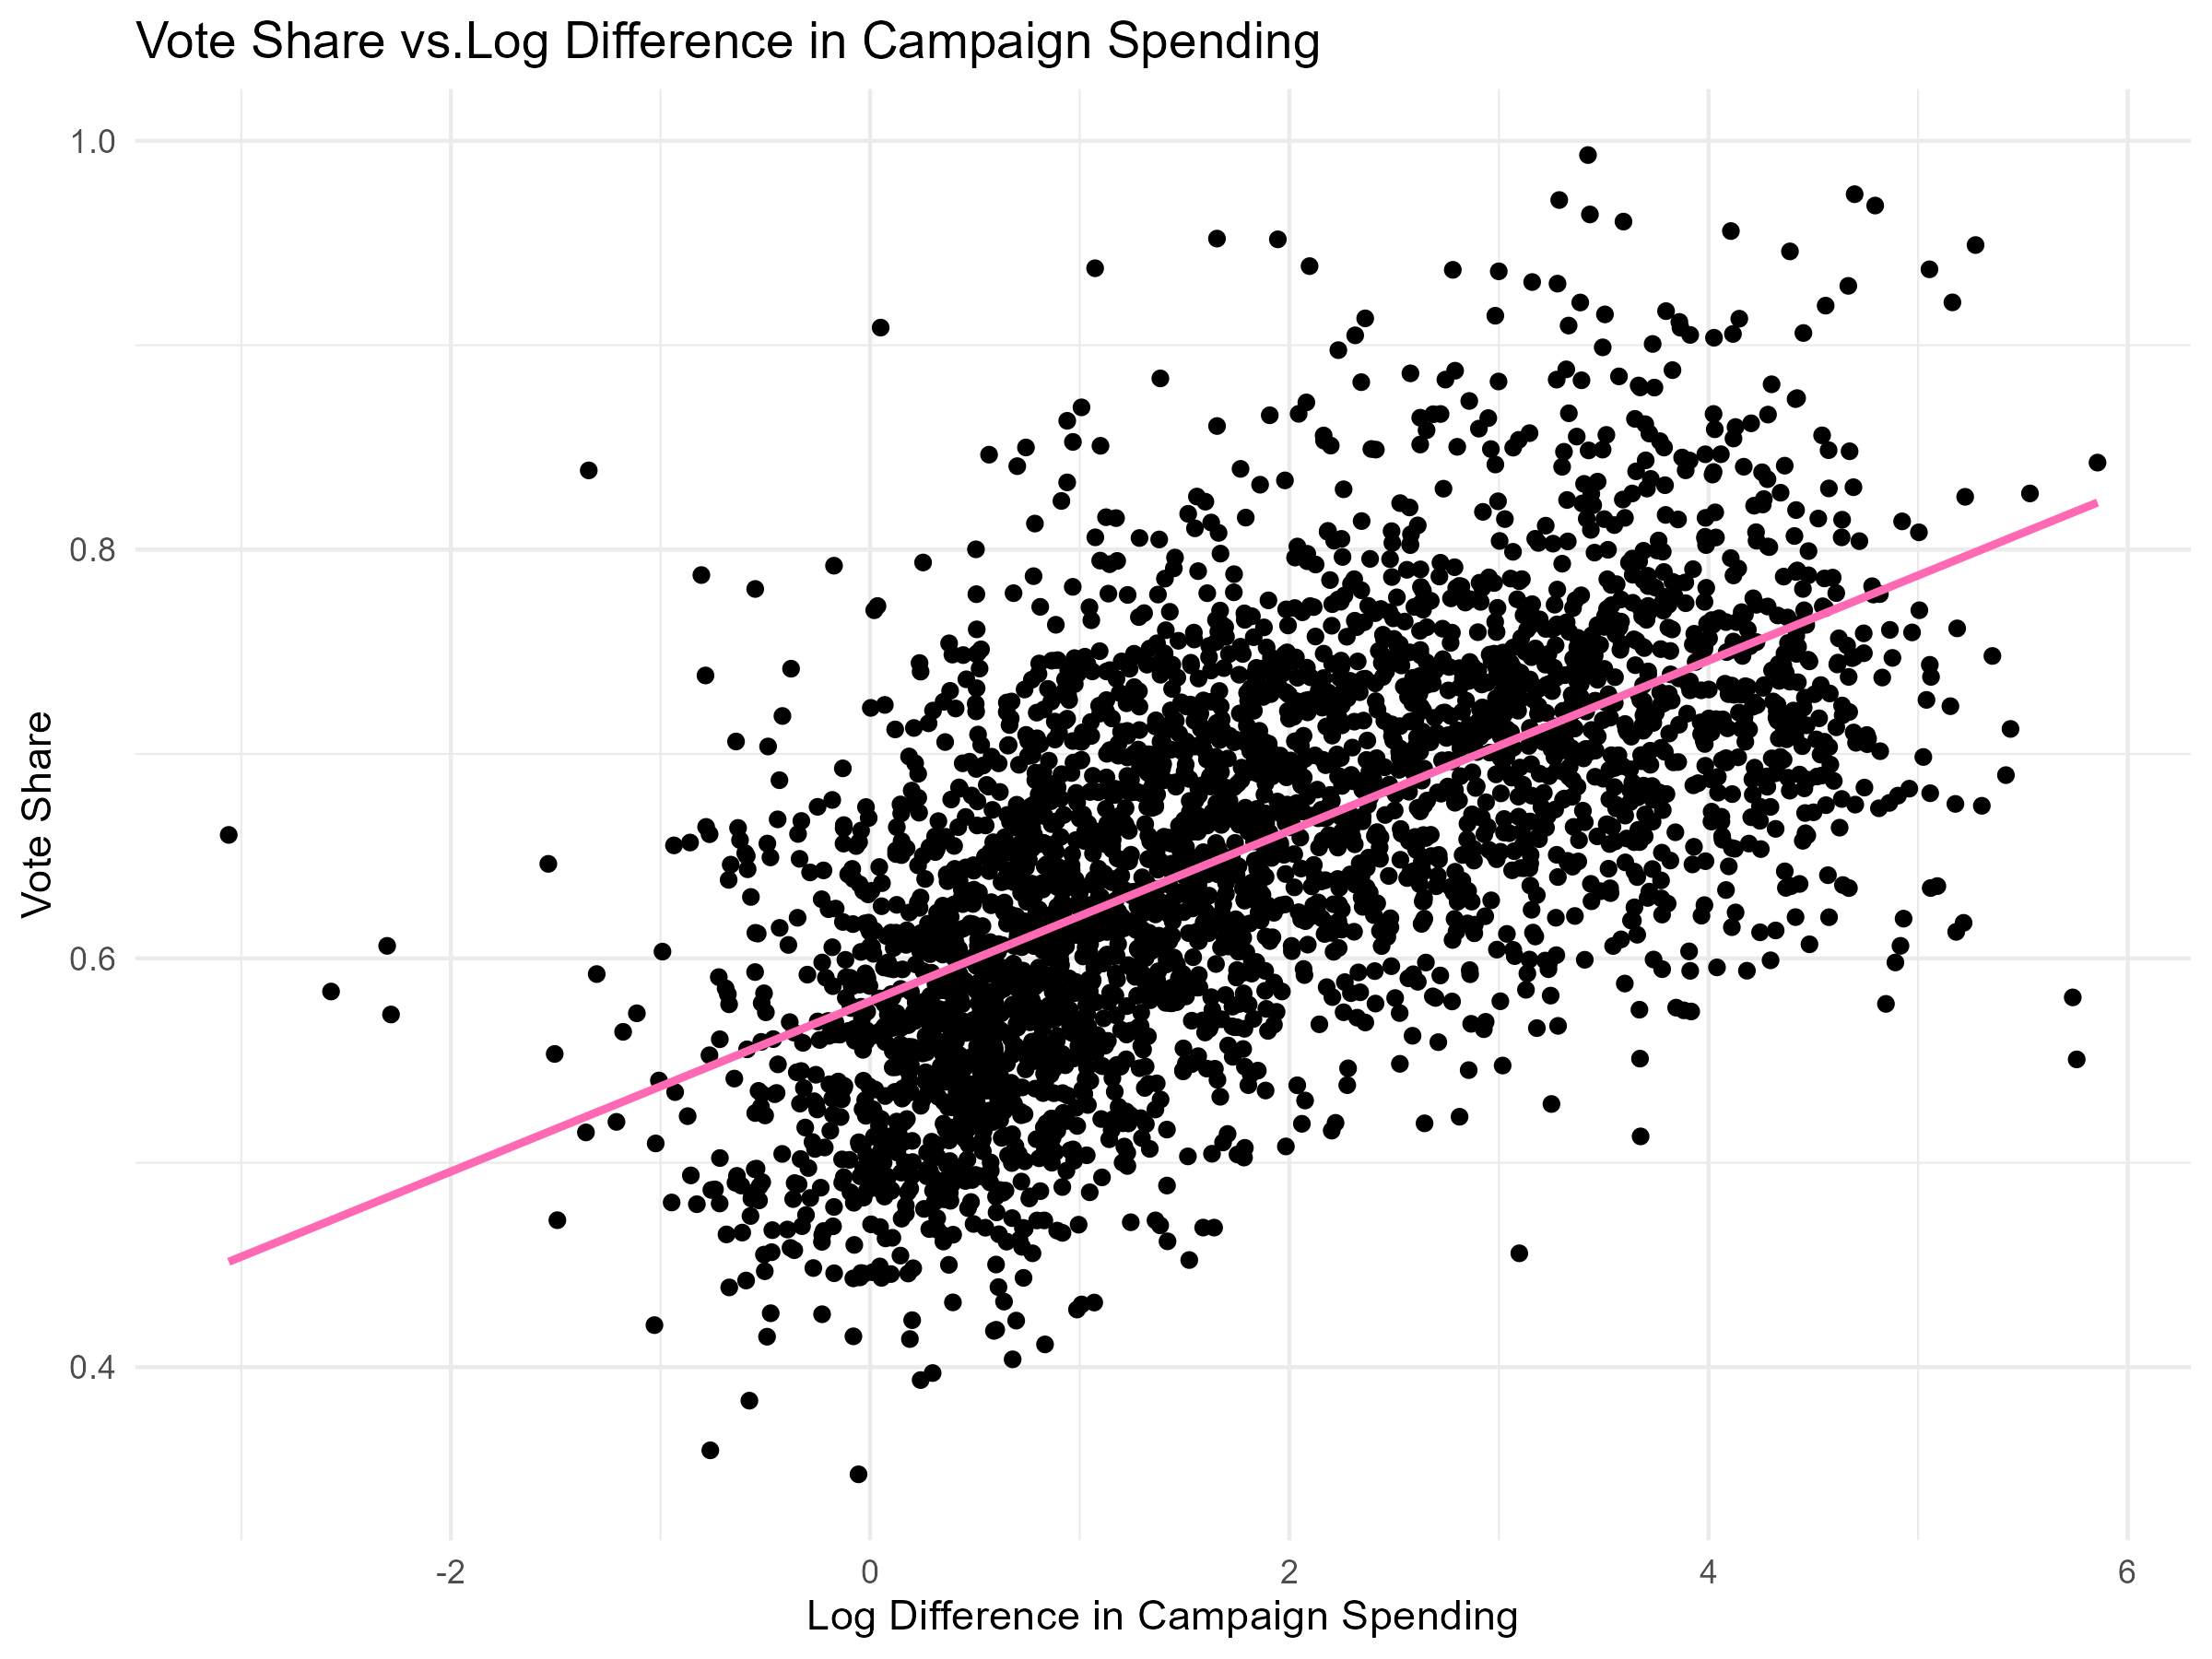
\includegraphics[width=0.8\textwidth]{scatter_dif_vote.png}
			\label{fig:scatter_dif_vote}
		\end{figure}
		\noindent This graph shoes a moderate positive correlation between the vote share and the Logarithmic difference in campaign spending.
		\lstinputlisting[
		language=R,
		linerange=start_q1.2-end_q1.2, includerangemarker=false,
		]{PS03 _answersAS.R}	
		\vspace{2cm}
		\item Save the residuals of the model in a separate object.
		\lstinputlisting[
		language=R,
		linerange=start_q1.3-end_q1.3, includerangemarker=false,
		]{PS03 _answersAS.R}
		\begin{lstlisting}
			> summary(residuals_lm1)
			Min.   1st Qu.    Median      Mean   3rd Qu.      Max. 
			-0.268319 -0.053454 -0.003769  0.000000  0.047798  0.327488 
		\end{lstlisting}
			\vspace{2cm}
		\item Write the prediction equation.
		\begin{equation}
			y = 0.579031 + 0.041666x
		\end{equation}
		\noindent{In the above prediction equation, y is equal to the predicted vote share and x is equal to the logarithmic difference in campaign spending between the incumbent and the challenger. Using this equation, it can be determined that, on average, there is a .041666 unit increase in the predicted vote share for every one unit increase in logarithmic difference in campaign spending. When there is no logarithmic difference in campaign spending (x=0), the vote share is 0.579031. }
	\end{enumerate}
	
\newpage

\section*{Question 2}
\noindent We are interested in knowing how the difference between incumbent and challenger's spending and the vote share of the presidential candidate of the incumbent's party are related.	\vspace{.25cm}
	\begin{enumerate}
		\item Run a regression where the outcome variable is \texttt{presvote} and the explanatory variable is \texttt{difflog}.
		\lstinputlisting[
		language=R,
		linerange=start_q2.1-end_q2.1, includerangemarker=false,
		]{PS03 _answersAS.R}
		\begin{lstlisting}
			
			Call:
			lm(formula = presvote ~ difflog, data = inc.sub)
			
			Residuals:
			Min       1Q   Median       3Q      Max 
			-0.32196 -0.07407 -0.00102  0.07151  0.42743 
			
			Coefficients:
			Estimate Std. Error t value Pr(>|t|)    
			(Intercept) 0.507583   0.003161  160.60   <2e-16 ***
			difflog     0.023837   0.001359   17.54   <2e-16 ***
			---
			
			Residual standard error: 0.1104 on 3191 degrees of freedom
			Multiple R-squared:  0.08795,	Adjusted R-squared:  0.08767 
			F-statistic: 307.7 on 1 and 3191 DF,  p-value: < 2.2e-16
		\end{lstlisting}
			\vspace{2cm}
		\item Make a scatterplot of the two variables and add the regression line. 
		\begin{figure}[h]
			\centering
			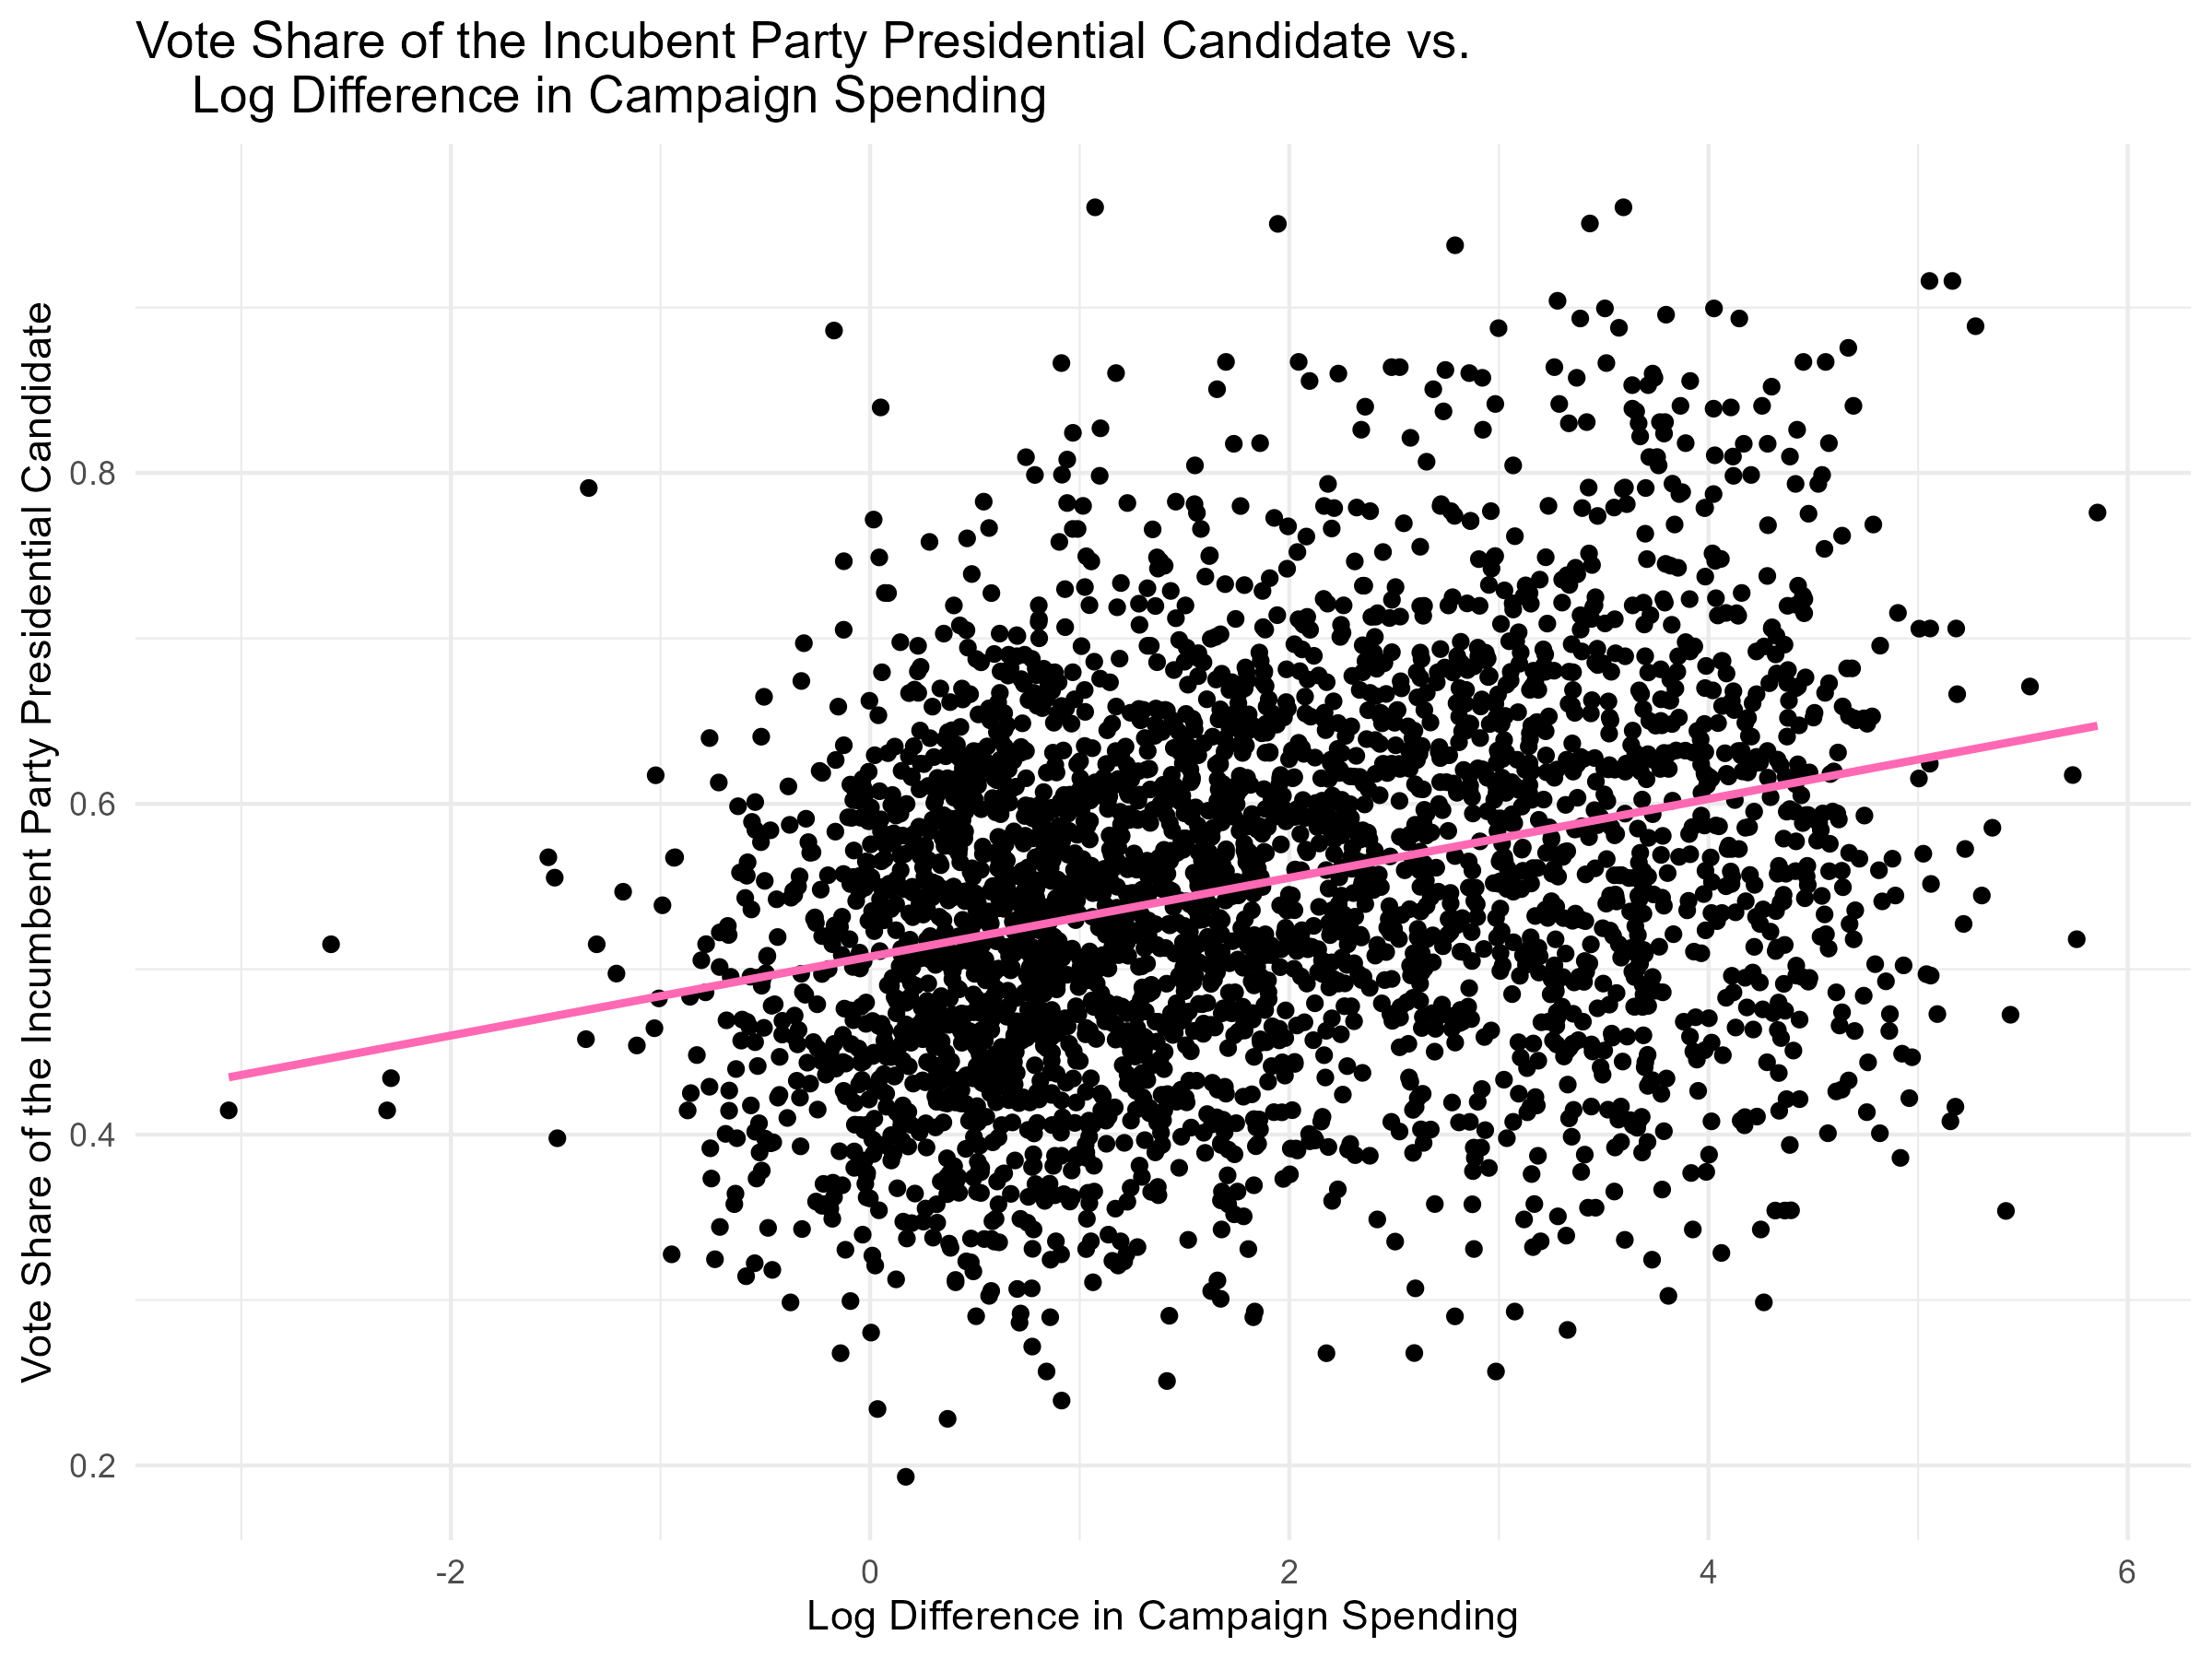
\includegraphics[width=0.8\textwidth]{scatter_dif_pres.png}
			\label{fig:scatter_dif_pres}
		\end{figure}	
		\lstinputlisting[
		language=R,
		linerange=start_q2.2-end_q2.2, includerangemarker=false,
		]{PS03 _answersAS.R}
		\noindent This graph shows a weak positive correlation between vote share of the incumbent party's presidential candidate and the logarithmic difference in campaign spending. 
		\vspace{2cm}
		\item Save the residuals of the model in a separate object.	\vspace{2cm}
		\lstinputlisting[
		language=R,
		linerange=start_q2.3-end_q2.3, includerangemarker=false,
		]{PS03 _answersAS.R}
		\begin{lstlisting}
			> summary(residuals_lm2)
			Min.   1st Qu.    Median      Mean   3rd Qu.      Max. 
			-0.321965 -0.074069 -0.001018  0.000000  0.071507  0.427435 
		\end{lstlisting}
		\item Write the prediction equation.
		\begin{equation}
			y = 0.507583 + 0.023837x
		\end{equation}
		\noindent{In the above prediction equation, y is equal to the predicted vote share of the presidential candidate of the incumbent's party and x is equal to the logarithmic difference in campaign spending between the incumbent and the challenger. Using this equation, it can be determined that, on average, there is a 0.023837 unit increase in the predicted vote share for the presidential candidate of the incumbent's party for every one unit increase in logarithmic difference in campaign spending. When there is no logarithmic difference in campaign spending (x=0), the vote share is 0.507583. }
	\end{enumerate}
	
	\newpage	
\section*{Question 3}

\noindent We are interested in knowing how the vote share of the presidential candidate of the incumbent's party is associated with the incumbent's electoral success.
	\vspace{.25cm}
	\begin{enumerate}
		\item Run a regression where the outcome variable is \texttt{voteshare} and the explanatory variable is \texttt{presvote}.
		\lstinputlisting[
		language=R,
		linerange=start_q3.1-end_q3.1, includerangemarker=false,
		]{PS03 _answersAS.R}
		\begin{lstlisting}
		
		Call:
		lm(formula = voteshare ~ presvote, data = inc.sub)
		
		Residuals:
		Min       1Q   Median       3Q      Max 
		-0.27330 -0.05888  0.00394  0.06148  0.41365 
		
		Coefficients:
		Estimate Std. Error t value Pr(>|t|)    
		(Intercept) 0.441330   0.007599   58.08   <2e-16 ***
		presvote    0.388018   0.013493   28.76   <2e-16 ***
		---
	
		Residual standard error: 0.08815 on 3191 degrees of freedom
		Multiple R-squared:  0.2058,	Adjusted R-squared:  0.2056 
		F-statistic:   827 on 1 and 3191 DF,  p-value: < 2.2e-16
		\end{lstlisting}
			\vspace{2cm}
		\item Make a scatterplot of the two variables and add the regression line. 
		\begin{figure}[h]
			\centering
			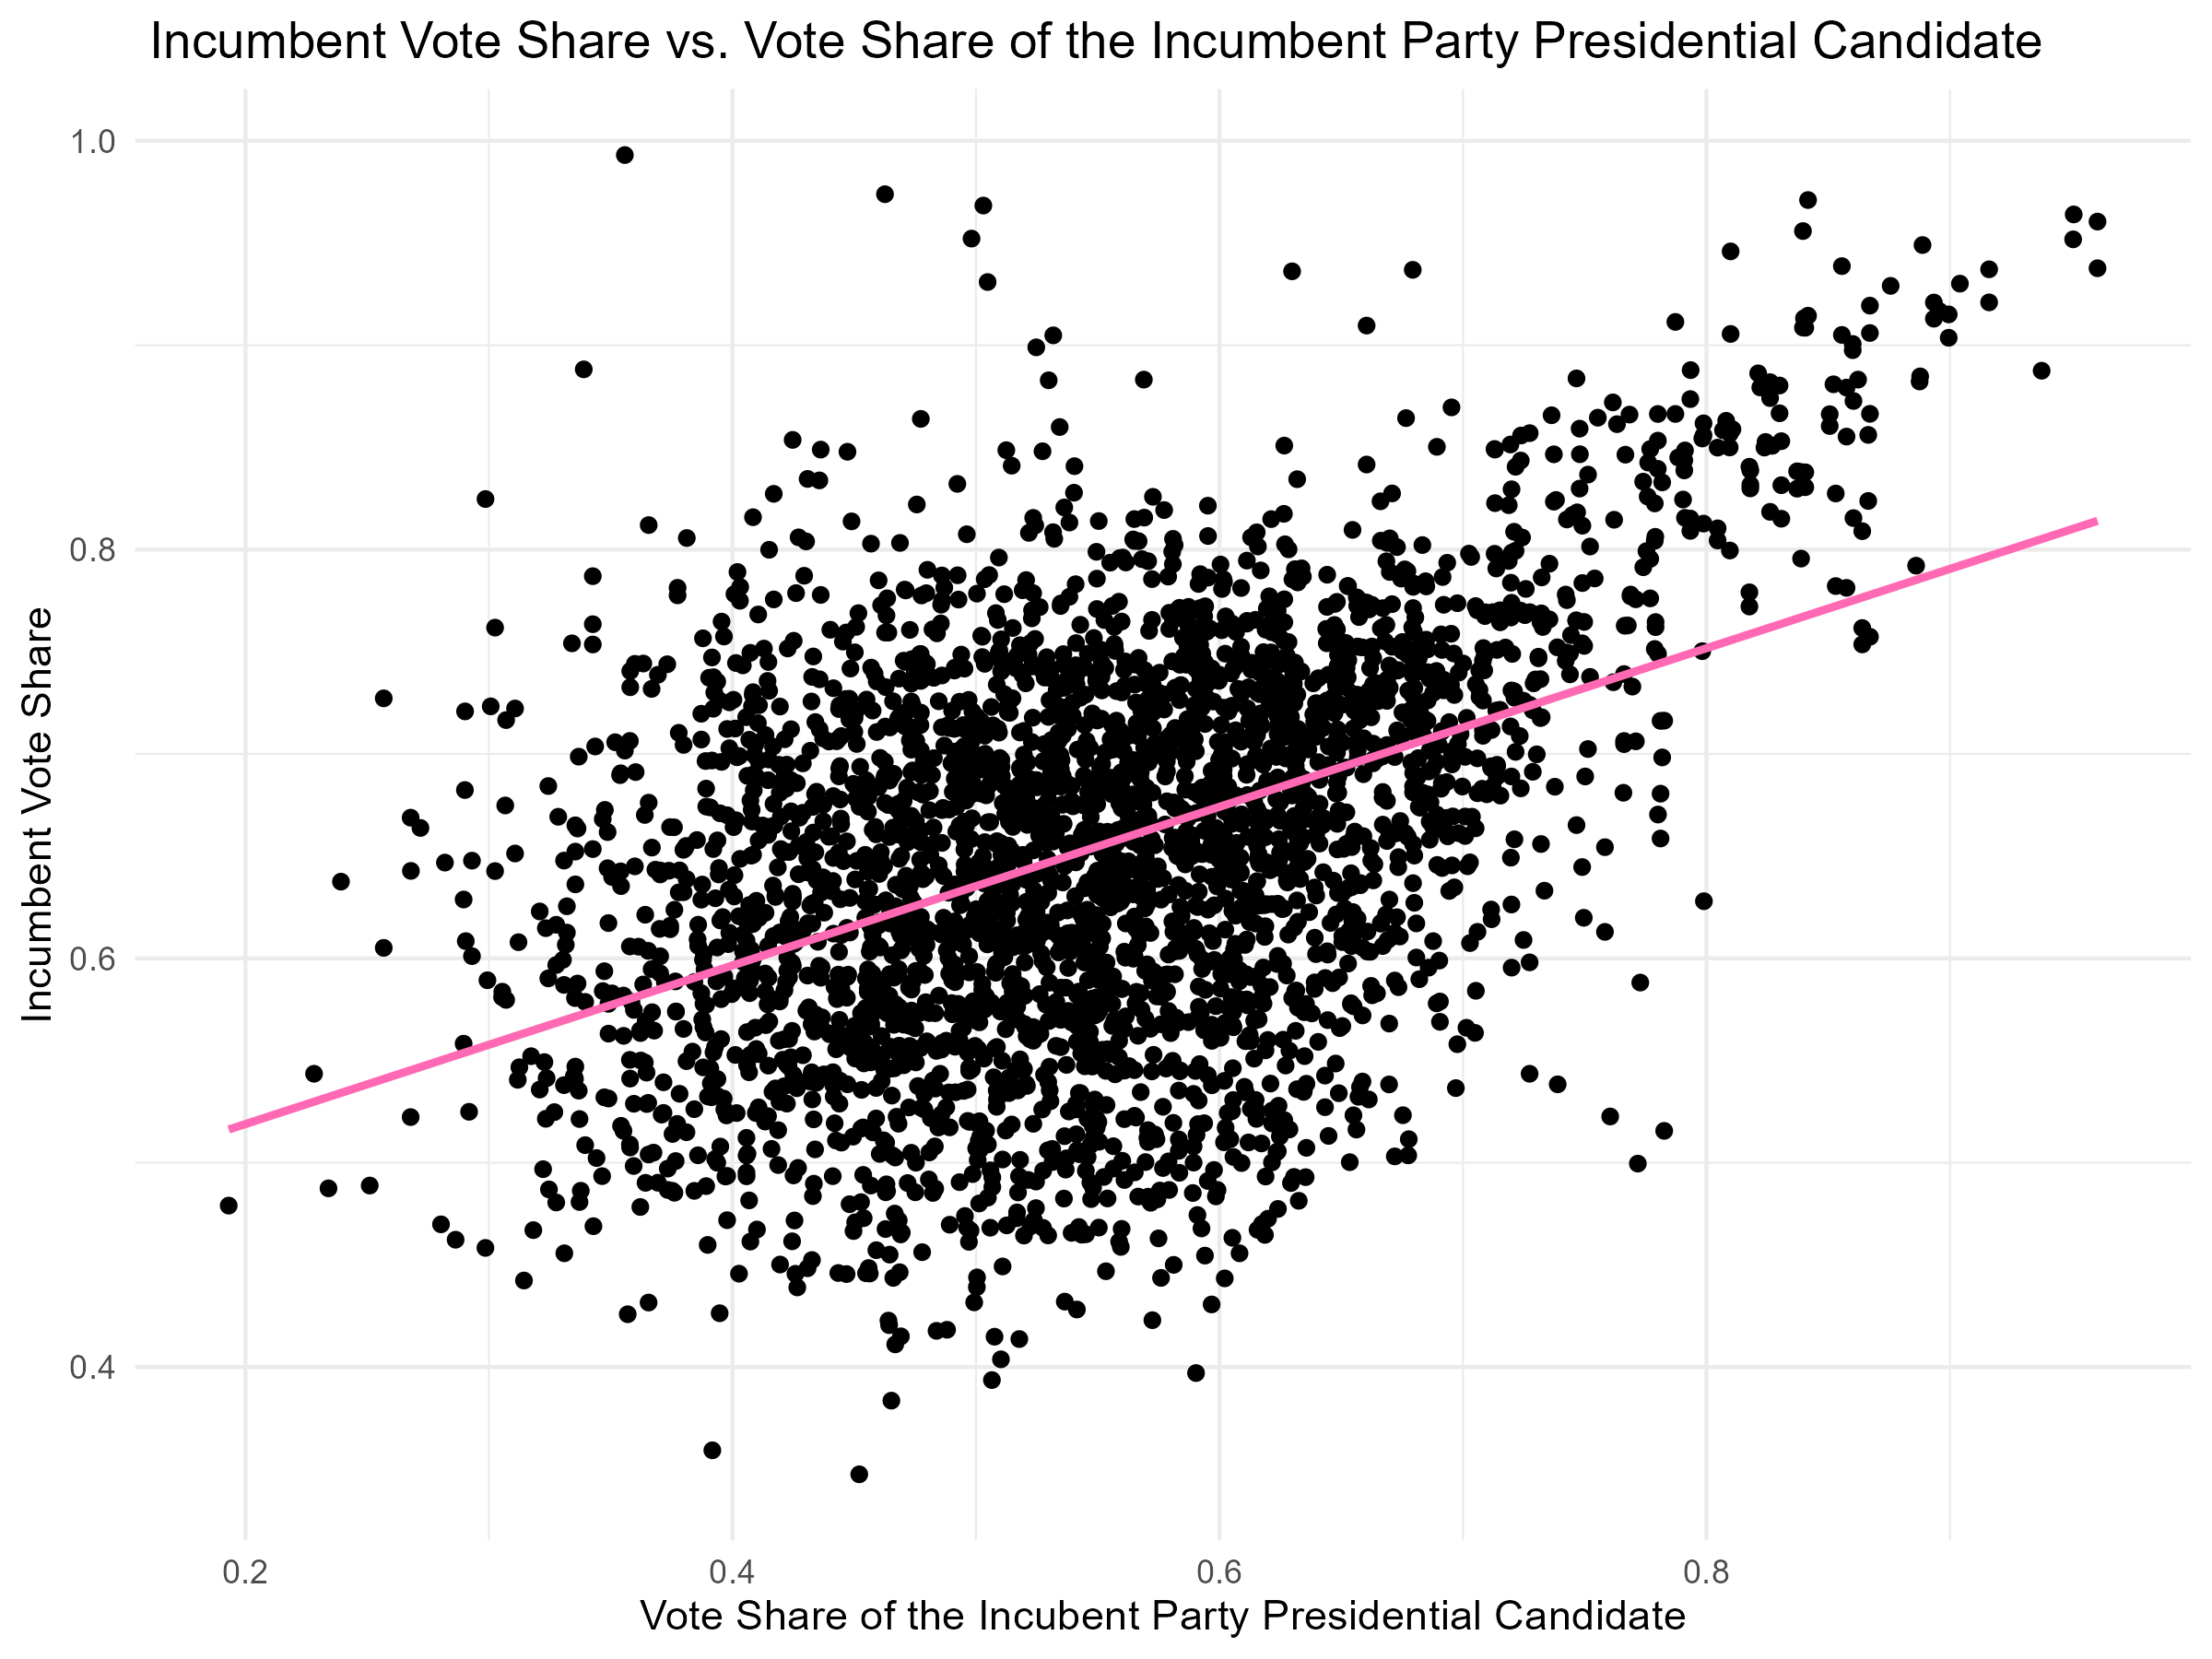
\includegraphics[width=0.8\textwidth]{scatter_pres_vote.png}
			\label{fig:scatter_pres_vote}
		\end{figure}	
		\lstinputlisting[
		language=R,
		linerange=start_q3.2-end_q3.2, includerangemarker=false,
		]{PS03 _answersAS.R}
		\noindent This graph shows a moderate positive relationship between the vote share of the presidential candidate of the incumbent's party  and the vote share.
			\vspace{2cm}
		\item Write the prediction equation.
		\begin{equation}
			y = 0.441330 + 0.388018x
		\end{equation}
		\noindent In the prediction equation above, y is the predicted incumbent's vote share and x is the vote share of the presidential candidate of the incumbent's party. On average, a one-unit increase in the presidential candidate's vote share is associated with a 0.388018 unit increase in the incumbent's predicted vote share.  When the presidential candidate's vote share is zero (x=0), the predicted incumbent vote share is 0.441330.
	\end{enumerate}
	

\newpage	
\section*{Question 4}
\noindent The residuals from part (a) tell us how much of the variation in \texttt{voteshare} is $not$ explained by the difference in spending between incumbent and challenger. The residuals in part (b) tell us how much of the variation in \texttt{presvote} is $not$ explained by the difference in spending between incumbent and challenger in the district.
	\begin{enumerate}
		\item Run a regression where the outcome variable is the residuals from Question 1 and the explanatory variable is the residuals from Question 2.	
		\lstinputlisting[
		language=R,
		linerange=start_q4.1-end_q4.1, includerangemarker=false,
		]{PS03 _answersAS.R}
		\begin{lstlisting}
			Call:
			lm(formula = residuals_lm1 ~ residuals_lm2)
			
			Residuals:
			Min       1Q   Median       3Q      Max 
			-0.25928 -0.04737 -0.00121  0.04618  0.33126 
			
			Coefficients:
			Estimate Std. Error t value Pr(>|t|)    
			(Intercept)   -5.934e-18  1.299e-03    0.00        1    
			residuals_lm2  2.569e-01  1.176e-02   21.84   <2e-16 ***
			---
			Residual standard error: 0.07338 on 3191 degrees of freedom
			Multiple R-squared:   0.13,	Adjusted R-squared:  0.1298 
			F-statistic:   477 on 1 and 3191 DF,  p-value: < 2.2e-16
			
		\end{lstlisting}
		\vspace{2cm}
		\item Make a scatterplot of the two residuals and add the regression line. 
		\begin{figure}[h]
			\centering
			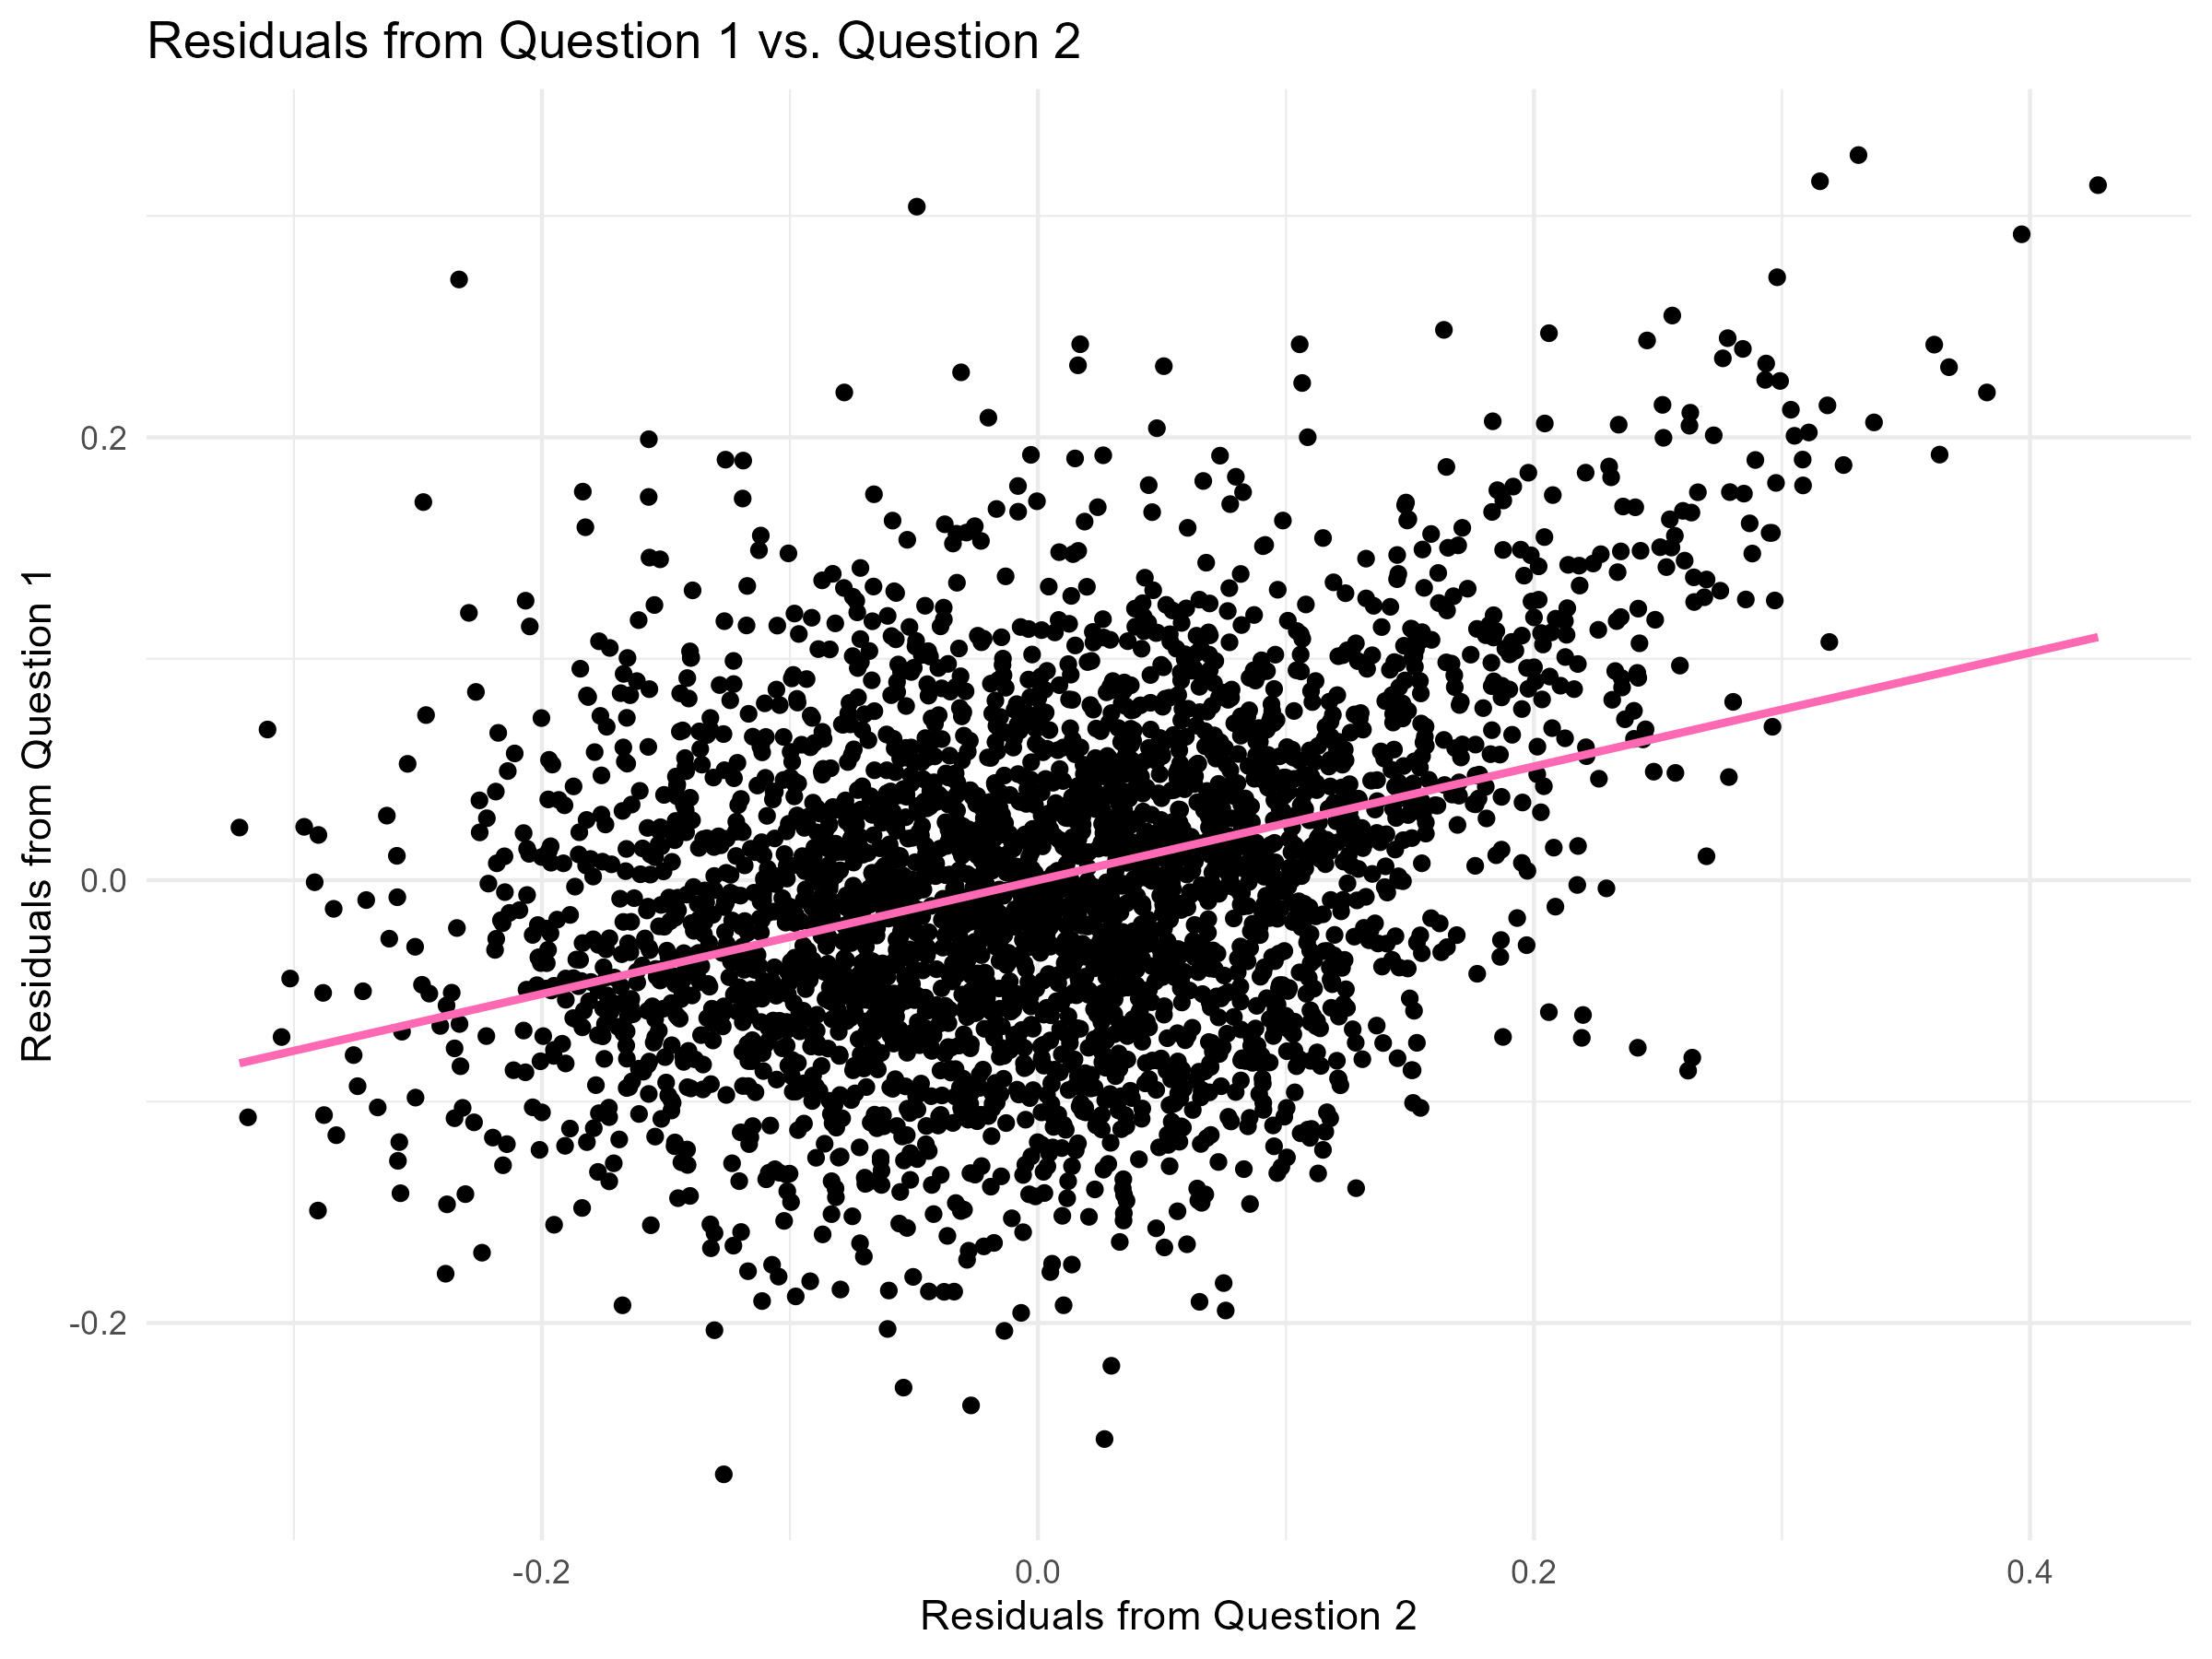
\includegraphics[width=0.8\textwidth]{scatter_residuals.png}
			\label{fig:scatter_residuals}
		\end{figure}	
		\lstinputlisting[
		language=R,
		linerange=start_q4.2-end_q4.2, includerangemarker=false,
		]{PS03 _answersAS.R}
		\ This graph shows a weak positive correlation between the residuals from question one and the residuals from question 2. 	\vspace{2cm}
		\item Write the prediction equation.
		\begin{equation}
			y = -5.934 \times 10^{-18} + 0.2569x
		\end{equation}
		\noindent In the above prediction equation, y is equal to the predicted residuals of the incumbent's vote share (or the variation in incumbent vote share not explained by spending) and x is equal to the residuals of the presidential vote share of the incumbent's party (or the variation in presidential vote share not explained by spending). On average, there is a 0.2569 unit increase in the predicted residuals of the incumbent's vote share for every one unit increase in the residuals of presidential vote share. When the residuals of presidential vote share are zero (x = 0), the predicted residuals of the incumbent's vote share are approximately zero (y=-5.934 x $10^{-18}$ ).
	\end{enumerate}
	
	\newpage	

\section*{Question 5}
\noindent What if the incumbent's vote share is affected by both the president's popularity and the difference in spending between incumbent and challenger? 
	\begin{enumerate}
		\item Run a regression where the outcome variable is the incumbent's \texttt{voteshare} and the explanatory variables are \texttt{difflog} and \texttt{presvote}.
		\lstinputlisting[
		language=R,
		linerange=start_q5.1-end_q5.1, includerangemarker=false,
		]{PS03 _answersAS.R}
		\begin{lstlisting}
			Call:
			lm(formula = voteshare ~ difflog + presvote, data = inc.sub)
			
			Residuals:
			Min       1Q   Median       3Q      Max 
			-0.25928 -0.04737 -0.00121  0.04618  0.33126 
			
			Coefficients:
			Estimate Std. Error t value Pr(>|t|)    
			(Intercept) 0.4486442  0.0063297   70.88   <2e-16 ***
			difflog     0.0355431  0.0009455   37.59   <2e-16 ***
			presvote    0.2568770  0.0117637   21.84   <2e-16 ***
			---
			Residual standard error: 0.07339 on 3190 degrees of freedom
			Multiple R-squared:  0.4496,	Adjusted R-squared:  0.4493 
			F-statistic:  1303 on 2 and 3190 DF,  p-value: < 2.2e-16
		\end{lstlisting}
		\vspace{2cm}
		\item Write the prediction equation.
		\begin{equation}
			y = 0.4486442 + 0.0355431x_1 + 0.2568770x_2
		\end{equation}	
		\noindent In the equation above y is the predicted vote share, $x_1$ is the logarithmic difference in spending between the incumbent and the challenger, and $x_2$ is the presidential vote share. on average, when the difference in spending and the presidential vote share are both zero ($x_1 = 0$ and $x_2 = 0$) the predicted vote share is 0.4486442 or 44.86\%. On average, for every one unit increase in the presidential vote share there is a 0.2568770 unit increase in the predicted vote share, holding the difference in spending constant. On average for every one unit increase in the logarithmic difference in campaign spending there is a 0.0355431 increase of in the predicted vote share, holding presidential vote share constant.
		 \vspace{2cm}
		\item What is it in this output that is identical to the output in Question 4? Why do you think this is the case?\vspace{.5cm}
		
		\noindent For both regressions, the distribution of the residuals (minimum, first quartile, median, third quartile, and maximum) are identical. Additionally, the residual standard error are the same. This is because the regression in Question 4 removes the influence of difflog from both voteshare and presvote before examining their relationship. In other words, it examines the variation in incumbent vote share that cannot be explained by spending and compares it to the variation in presidential vote share that cannot be explained by spending. The multiple regression in Question 5 does this by including both difflog and presvote as independent variables, effectively holding the difference in campaign spending constant. Therefore, the two regressions are accounting for the same variations.
	\end{enumerate}




\end{document}
